\documentclass[12pt]{article} 
\usepackage[utf8x]{inputenc} 
\usepackage{amsmath} 
\usepackage{multicol} 
\usepackage{graphicx} 
\usepackage{float} 
\usepackage[sorting=none]{biblatex}
\bibliography{bibs.bib}
\usepackage{dsfont} 
\usepackage{textcomp} 
\usepackage{multirow} 
\usepackage{amsfonts} 
\usepackage[colorlinks=True]{hyperref}
\hypersetup{linkcolor=black,
citecolor=blue}
\usepackage{cleveref} 
\usepackage{fancyhdr} 
\setlength{\headheight}{14.5pt} 
\renewcommand{\sectionmark}[1]{\markright{#1}{}} 
\usepackage[T1]{fontenc} 
\usepackage[colorinlistoftodos]{todonotes} 
\usepackage[margin=2cm,a4paper]{geometry} 
\newgeometry{left=2.0cm,right=2.0cm,top=2.5cm,bottom=2.0cm} 
\usepackage{listings}
\setlength{\marginparwidth}{2cm} 
\usepackage[onehalfspacing]{setspace}
\setlength{\parindent}{0pt} 
\newcommand{\deriv}{\mathrm{d}} 
\title{} 
\pagestyle{fancy} 
\fancyhf{} 
\rhead{\leftmark} 
\lhead{Very Near Sun Exploration} 
\rfoot{Page \thepage} 
\renewcommand{\headrulewidth}{1pt} 
\renewcommand{\footrulewidth}{1pt} 
\begin{document}
%--------------------------------------------------------------------------------
%	TITLE PAGE
%--------------------------------------------------------------------------------
\begin{titlepage}
\newgeometry{left=1.0in,right=1.0in,top=2.0in,bottom=1.0in}
\newcommand{\HRule}{\rule{\linewidth}{0.5mm}}
\begin{centering} 
%---------------------------------------------------------------------------
%	HEADING SECTIONS
%---------------------------------------------------------------------------

\includegraphics[scale=0.6]{Media/Document/Uni_of_Kent.png}\\
%---------------------------------------------------------------------------
%	TITLE SECTION
%---------------------------------------------------------------------------
\vspace{1.0cm} 
\large{\emph{Division of Natural Sciences, University of Kent in Canterbury}} \\ [0.1cm]
\large{Department of Physical Sciences, Ingram Building} \\ [1.0cm]
\Huge{\bfseries{Magnox Radioactive Waste \\ Disposal Container}} \\ [1.0cm]
{\Large \bfseries{By \\ [0.2cm] Lukasz R Tomaszewski}}\\[0.2cm]
\textsc{\large BSc (Hons) Astronomy, Space Science and Astrophysics}\\ [-0.2cm]
\textsc{\large PH617: Physics Project Laboratory}\\ [-0.2cm]
\textsc{\large Word Count: 6260 (LaTeX)}\\ [1.5cm]
{\Large \bfseries{March 2021}}\\
\end{centering} 
\end{titlepage}
%---------------------------------------------------------------------------
\newpage
\begin{titlepage}
\begin{tableofcontents}
\end{tableofcontents}
\end{titlepage}
\newpage

%--------------------------------------------------------------------------- 
%	ABSTRACT
%--------------------------------------------------------------------------- 

\section{Abstract} 
\label{Abstract}

The Solar Orbiter probe is currently the only probe designed to observe the Sun at 0.28AU from its surface, the closest man-made probe ever to orbit the Sun. In this project we discuss the possibility of a mission that travels within 0.2AU of the Sun's surface. To do so, a future probe must be protected by a heat shield manufactured from titanium alloys and thermoresistant materials to withstand the temperature of the Sun and be powered by an on-board electrical power unit that assists the solar panels. The probe can send data via radio or a laser that incorporates PPM (pulse position modulation) to combat the interference from the Sun and Earth's atmosphere, such data can include: the ionization of the Sun’s atmosphere, the effect and shape of the Sun's magnetosphere and data on the Sun’s coronal activity. Faraday cups, magnetometers, thermal gauges, X-ray/UV sensors and other instruments must be installed alongside the power units, data transmitters and other on-board systems, and sensors that are encased in the probes hull. These must be able to withstand  hazards of space travel such as the Sun's temperature and solar flares, and space debris. The probe is fitted with redundancy systems as the probe must be largely independent as it travels through space and orbits the Sun. 

%--------------------------------------------------------------------------- 
%	INTRODUCTION 
%--------------------------------------------------------------------------- 

\section{Introduction and Background} \label{Introduction}

The purpose of this report is to discuss the prospect of a space mission to explore the very near-Sun environment. Although the Sun has for millennia been an object of human curiosity and investigation, much is still unknown about its mechanics and dynamic environment. In order to fully understand the near-Sun environment, it is not enough to take measurements from Earth - the probe must travel to the Sun. For example, by the time solar winds reach us on earth, they are too diffuse to properly understand their origins. Here, very near-Sun means between a mission that travels within 0.2AU of the Sun's surface. Ideally, the mission would come even closer to the sun, in order to surpass the achievement of the Parker Solar Probe, which will in 2025 hold the current record for closest approach to the Sun at 9.86 solar radii \cite{parkerpresskit}. This will mean the probe must travel within the Sun's atmosphere, where temperatures reach well over 1,000 degrees Celsius. This poses a great challenge in terms of probe design and materials. Sensitive equipment must be properly shielded from the intense radiation, and communications technology must account for the extremely close proximity to the Sun, which may interfere with transmission. 

\vspace{\baselineskip}

Due to time constraints and the huge potential breadth of this task, the scope of this project will be somewhat limited. It will focus on the thermal challenges presented by the near-Sun environment, communications technologies, and instrumentation required on board. It will evaluate what data to be collected will provide the most scientific and economic value, in order to justify the high cost of such a mission. Some topics that would in reality be essential are not discussed, for example propulsion and costing. Section \ref{data} will discuss unanswered questions about our Sun, and what data could potentially be gathered to resolve these questions. It will also discuss the economic incentives in terms of understanding damaging space weather for the mission. Section \ref{Instrumentation} will discuss the equipment necessary to achieve these aims. Section \ref{Communications} will explore how the data collected can be transmitted back to Earth. Section \ref{The Near-Sun Environment} will discuss the environment the probe will encounter near to the Sun, and section \ref{Materials} will explore the materials that can be used on the probe which can be used to protect it from this harsh environment.

\subsection{History of Solar Missions}

The following section provides a brief history of previous solar investigation space missions, the first of which was the NASA Pioneer 5, launched in 1960, and the most recent being the ESA Solar orbiter, launched in February 2020. 

\vspace{\baselineskip}
\textbf{NASA Pioneer Missions}
\vspace{\baselineskip}

Launched in 1960, the Pioneer 5's mission was to investigate the magnetic field in interplanetary space. The mission was a success - the probe confirmed the presence of these interplanetary fields. It also observed solar flare particles and cosmic radiation \cite{pioneer5}. It was equipped with a telescope, magnetometer, ionization chamber and momentum spectrometer \cite{pioneerinstruments}. Five further Pioneer probes were launched during the 60's, the last of which, Pioneer E, failed to reach orbit. The other probes gathered information about: "the solar wind, solar cosmic rays, the structure of the Sun's plasma and magnetic fields, the physics of particles in space, and the nature of storms on the Sun which produce solar flares" \cite{pioneers}.

\vspace{\baselineskip}
\textbf{NASA/ESA Ulysses}
\vspace{\baselineskip}

The Ulysses, launched in 1990, lasted four times as long as was expected, with contact only lost as of June 2009. The Ulysses unexpectedly encountered the comet Hyakutake, discovering that comet tails were far longer than was expected, whilst the Sun's magnetic field was weaker than expected. It also determined that the magnitude of the Sun's solar wind was declining \cite{ulysses}. 

\vspace{\baselineskip}
\textbf{NASA/ESA SOHO}
\vspace{\baselineskip}

Despite only being planned to last 2 years, the Solar and Heliospheric Observatory project has been renewed several times since its launch in 1995, most recently to 2020. It is expected to be renewed again to 2022 \cite{sohoextension}. It was built by a consortium led by Matra Marconi Space, now Airbus Defence and Space. The probe orbits the First Lagrangian Point, around 1.5 million kilometres away from Earth. Its ongoing mission is to investigate solar activity, weather, and magnetic field. The knowledge gained from this mission has provided insight into the structure of sunspots and the solar interior. It also acts as a 3 day space weather early warning system. So far it has detected more than 2000 new comets, and new solar phenomena such as coronal waves and solar tornadoes \cite{soho}.

\vspace{\baselineskip}
\textbf{NASA Parker Solar Probe}
\vspace{\baselineskip}

The Parker Solar Probe, launched on 12th August 2018, is an ongoing space mission designed to observe and measure the environment closer to the Sun and improve the forecasting of destructive and hazardous space weather. The probe, shown in figure \ref{psp_diagram}, will perform several Venus flybys while in its heliocentric orbit to reduce its orbital speed. It aims to investigate why the Sun’s corona (atmosphere) is much hotter than its surface. 

\begin{figure}[H]
    \centering
    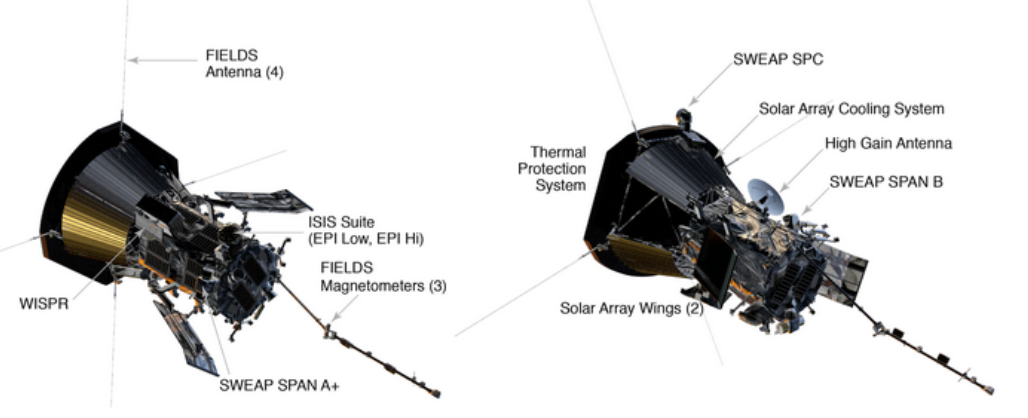
\includegraphics[width = 12cm]{Media/Document/psp.PNG}
    \caption{Parker Solar Probe, courtesy of GENIUS TOUR}
    \label{psp_diagram}
\end{figure}


\label{Introduction Section} 

 

%--------------------------------------------------------------------------- 

%	MISSION PURPOSE

%--------------------------------------------------------------------------- 
\section{Mission Purpose and Data Collection} \label{data}

It is important that the data to be collected justifies the cost of the mission. One way in which greater knowledge of the Sun could assist on Earth is in furthering our understanding of solar weather events. These weather events can interfere with Earth, or Earth orbit based equipment such as satellites. Substantial data has already been collected regarding the dynamics of the Sun, for example, data on the cause and effects of solar storms on Earth. However the complexities of these storms, and the precise mechanisms by which changes in the Sun's environment cause them, are not yet fully understood. A very near-Sun expedition will be able to collect more enlightening data on solar weather and perhaps allow us to make our equipment more resilient against these disturbances. 

The mission should therefore collect data on:

\begin{itemize}
    \item the Sun's changing magnetic field
    \item sunspots, using UV cameras
    \item radio shock waves created by coronal mass ejections (CME's) crashing into solar winds
\end{itemize}

CMEs occur in the Sun's corona, an area structured by strong magnetic fields. When these fields are closed over, often above groups of sunspots, the solar atmosphere is confined and these pockets of gas in the magnetic field pockets can suddenly and violently erupt. This releases bubbles of gas, resulting in an increase in magnetic field strength creating a coronal mass ejection. When this occurs, the solar material expelled can affect planetary bodies and satellites \cite{sundata}. These CMEs can push through the solar winds, and propagate in any direction, including towards Earth. The most significant issue when this occurs is the shocks formed at the front of the CME or solar flare. These cause the release of high velocity, charged solar energetic particles. They will follow the magnetic field lines that permeate the space between the Sun and Earth - some of which intersect with the Earth itself, causing damage and disruption \cite{spacweather}. The impacts result in the deterioration of microelectronics, optical components and solar cells in satellites. This can cause data to become corrupted, system to shutdown and even damage circuits \cite{seps}. Repairs can be extremely expensive, both monetarily and in terms of time - satellite damage is especially problematic as this may necessitate sending more equipment or man power into orbit, or decommissioning the technology and manufacturing a new satellite. 

\bigskip

The mission could collect spectroscopic images of the release of gas bubbles, to determine what gases are released, and how the releases correlate to CMEs. These ejections from the Sun’s corona are of such high temperatures that they produce UV and X-rays \cite{sundata}. This data may allow for the creation of models that can make predictions about when CMEs will occur. Magnetometers can also be used to examine the changes in the magnetic field. This data could help predict how large a given CME will be and the impact it will have on the planetary bodies towards which it is directed. Collecting detailed data from close proximity to the sun could also help understand the origin of the CMEs - whether they are a result of solar flares, or an independent event.

\vspace{\baselineskip}

Solar minima, times where the Sun has few sun spots, occur over a period of several years. Conversely, solar maxima are years where sunspots are most prominent, but their durations have been less well defined. They are estimated to take approximately 11 years \cite{sundata}. Collecting images of the fluctuating sunspots in various spectra (X-ray, gamma ray, UV, and visible) could allow for a better model of solar minima and maxima to be constructed. Such a model would allow for more accurate prediction of solar flares and CMEs.

\vspace{\baselineskip}


Solar maxima occur due to sudden changes in the Sun's magnetic polarity. These changes also cause solar flares, CMEs and sunspots. As the Sun, like Earth, rotates on its axis, its magnetic field also rotates in a large spiral pattern (The Parker Spiral). Therefore, solar storms affect objects across the solar system \cite{solatsystemdata}. Collecting data on the Sun's magnetic field would allow for earlier predictions of when these solar storms would occur. By monitoring the changes in the field, and its structure closer to the Sun's surface, we would better be able to model the rotating magnetic spirals during solar minima and maxima. This would help identify events that will effect electronics on earth and in space, so that equipment can be shut down to protect against power surges, as well as help in understanding other Sun-like stars. This would help us know how to equip future missions to other stars. 

\begin{figure}[H]
    \centering
    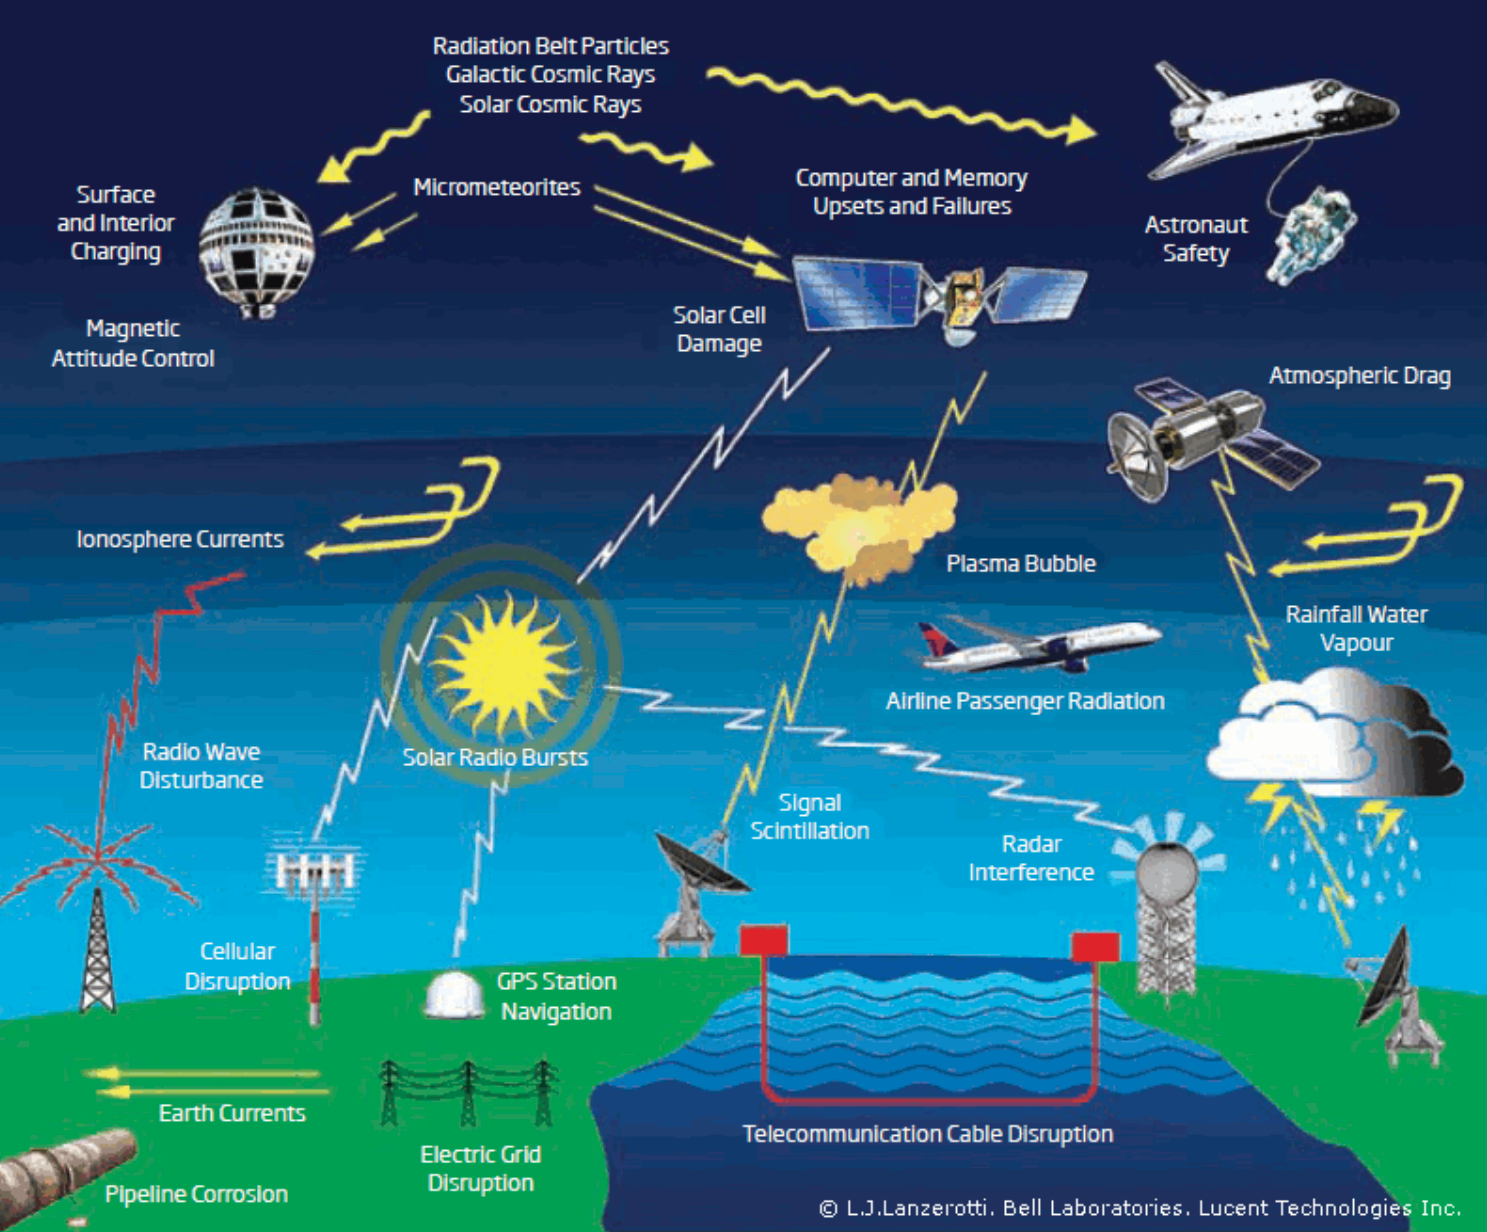
\includegraphics[width = 12cm]{Media/Document/weather.png}
    \caption{Illustration showing the effects that solar radiation has on the technologies of the Earth \cite{whatisweather}}
    \label{magnetometer_diagram}
\end{figure}

 Not only does solar weather pose a threat to electrical equipment, but the increased radiation flux on Earth could result in an increased number of radiation induced illnesses, such as cancers, with serious consequences including increased risk of mortality. Data gathered from particle detectors in space could allow for the preparation and adaptation of spacesuits, as astronauts would be the most at risk from the radiation when these events occur. 

\vspace{\baselineskip}

Temperature gauges could be used to monitor the change in surface temperature of the sun in various places. For example, where sunspots occur the temperature in the region of the spot is lower than the average surface temperature. Detecting these temperature changes would allow us to predict where sunspots will occur and whether this will result in solar flares or CMEs. Imaging in the UV and visible spectra already allows determination of the location of sunspots, but does not allow us to predict where sunspots will occur as early as we would like. By monitoring magnetic field fluctuations and temperature in the region between 0 and 0.2AU from the sun, it will be possible to determine where sunspots will occur, as the magnetic field fluctuations precipitating a sunspot result in a temperature drop from 6,000 to 4,200 degrees Celsius \cite{sundata}. This will help us form a predictive model.

\section{Instrumentation} \label{Instrumentation}

A space probe navigating towards the Sun consists of several essential components including its propulsion, power, navigation, communication and data handling systems, but its scientific payload is also of particular importance. The purpose of a probe’s mission is scientific study, but the number and complexity of its on board instruments and experiments are limited by mass. The scientific payload must therefore be both efficient and profitable in the pursuit of further knowledge and understanding of our solar system. These instruments can also be sensitive to external forces, hazardous phenomena and contamination unique to space and spaceflight, so every instrument must be uniquely tailored for the mission, which significantly increases costs.

\vspace{\baselineskip}
\subsection{Magnetometer}
\vspace{\baselineskip}

As detailed in section \ref{data}, taking magnetic field measurements will be essential. Magnetometers are devices which measure the magnitude, direction and change in magnetic fields over distance and time. There are two types of magnetometers used by space exploration missions, fluxgate magnetometers or FGMs and vector Helium magnetometers or VHMs. FGMs are very low mass, low power and capable of detecting low-frequency vector measurements. The FGMs installed in a probe’s scientific payload typically use a ring-shaped core of a few centimeters diameter with magnetic saturation oscillating between magnetised, unmagnetised, inversely magnetised, unmagnetised, magnetised and so on. This saturation is achieved by a periodic bi-polar current pulse in the drive winding looped around the ring. To detect an external magnetic field, a sense winding wound laterally around the core senses any electromagnetic induction produced by a change in flux and outputs a signal \cite{fluxgate}, \cite{whatisfluxgate}. This type of magnetometer is shown in figure \ref{magnetometer_diagram}. On the other hand, VHMs are better suited to high-frequency vector measurements and offer improved resolution and durability. These devices, occasionally used in tandem, are often mounted on booms to reduce magnetic contamination from the main body of the spacecraft \cite{magnetometers}.

\begin{figure}[H]
    \centering
    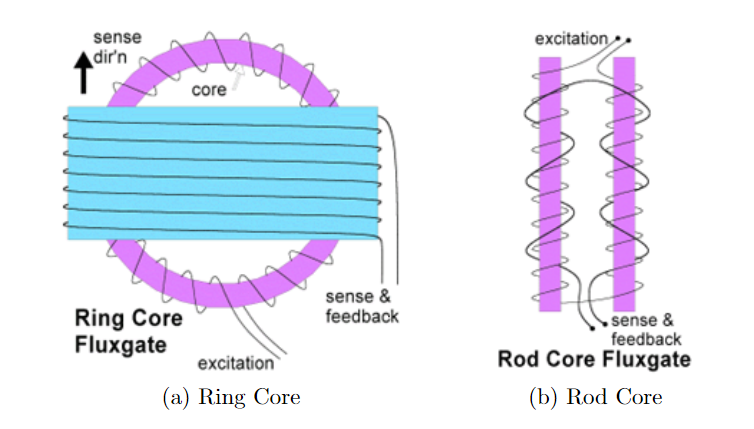
\includegraphics[width = 12cm]{Media/Document/magnetometer.PNG}
    \caption{Fluxgate magnetometers, courtesy of sensorland.com}
    \label{magnetometer_diagram}
\end{figure}


\vspace{\baselineskip}
\subsection{Faraday Cup}
\vspace{\baselineskip}

A Faraday cup is composed of a metal block or ‘cup’ designed to count the number of ions or electrons from a beam by measuring the current produced by the incident charge absorbed by the metal. Since the charge of an ion or electron is a known, discrete value and current is charge in Coulombs per second, the number of particles per second may be calculated from Equation 1:

\begin{equation} \label{particles}
    Ne = It
\end{equation}
\vspace{\baselineskip}
where e is the magnitude of the charge of an electron, $e = 1.6 × ^{−19} C$. 

The Solar Probe Cup or SPC, a component of the SWEAP suite on the Parker Solar Probe, is a Sun-pointing Faraday cup composed of refractory metals and sapphire crystal insulators \cite{faradaycup}. Its objective is to count the incident electrons, protons, alpha particles and solar wind ions while measuring their energy-dependent flow angles and one-dimensional velocity distribution functions \cite{pspcup}.

\vspace{\baselineskip}
\subsection{Mass Spectrometer}
\vspace{\baselineskip}

Mass spectrometry is the analytical process whereby the atoms of a sample are identified and quantified by their charge-to-mass ratio. The sample is first vaporised to free its atoms from their bonds and positively ionised by a beam of electrons, this accelerates them towards plates of negative potential with slits to focus the ions into a beam. These ions are subsequently deflected by a magnetic field according to their charge-to-mass ratio. The lighter the ion and the greater its charge, the greater the angle of its deflection. Some of the ions hit the walls of the spectrometer chamber and are thus unrecorded, while others strike the detector and generate an electric signal proportional to the count of the ions of one specific chemical element. The placement of the incident ions on the detector indicates their element. The mass spectrometer’s data system will typically output a plot of relative abundance of an ion against charge-to-mass ratio if sufficiently calibrated. The peaks on this plot represent the quantified presence of specific ions within the sample \cite{massspectrometer}.

\begin{figure}[H]
    \centering
    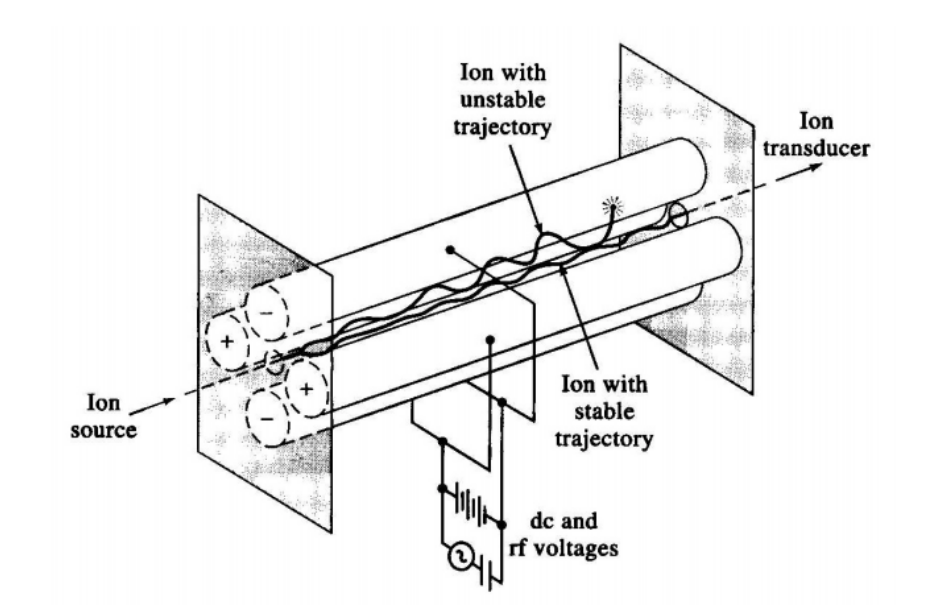
\includegraphics[width = 12cm]{Media/Document/massspectrometer.PNG}
    \caption{Quadrupole mass spectrometer, courtesy of University of Massachusetts Lowell}
    \label{mass_spectrometer_diagram}
\end{figure}


The mass spectrometers utilised by modern-day spacecraft include sophisticated analysers able to measure the chemical composition of matter in various states including plasma \cite{massspectrometry}. One type of mass spectrometer typically utilised in a probe’s scientific payload is a quadrupole mass spectrometer. These devices are composed of four magnetised rods displayed in figure \ref{mass_spectrometer_diagram}. The vaporised sample is ionised and funnelled into a beam by a slit before passing through the centre of the quadrupole arrangement. The magnetic fields of the rods divide the ions into multiple beams corresponding to their charge-to-mass ratios with each beam possessing a complex individual oscillating trajectory. Only the beams with stable trajectories strike the detector and are recorded by the data system. A quadrupole mass spectrometer is particularly useful in space applications because they can select the type of ions desired for measurement as well as what specific ion components to measure. This is useful in an environment with an abundance of free particles such as the Sun’s superheated corona. Furthermore, they are also more resistant to launch vibrations and extreme temperatures \cite{quadrapole}. 

\vspace{\baselineskip}
\subsection{Thermal Gauge}
\vspace{\baselineskip}

The probe’s computers and electronic systems produce thermal energy as a waste product and, together with the extreme thermal environment of the Sun’s corona, this can compromise the probe’s systems and instrumental data. A thermal gauge, which records the thermal energy of a homogeneous substance, is a central part of a probe’s thermal control system and assists in optimising operational conditions in real time. It alerts the rest of the system if the temperature rises or falls from an suitable range and quantifies potential thermal contamination. Thermistors are commonplace in temperature gauges and monitor temperature by measuring the proportional resistance through the component. This resistance increases with an increase in temperature and affects the output voltage signal.
\vspace{\baselineskip}

The thermistors utilised in deep-space missions are usually small, very sensitive and built to endure long mission durations. To reliably measure the temperature of the probe and its operations, the device must be close to the heat source and ideally within physical contact of it. There should also be more than one gauge in differing placements to gain accurate averaged readings, but also to pinpoint the sources of excess temperatures within the craft. In addition, the data from these devices may serve to improve future mission efficiencies.

\vspace{\baselineskip}
\subsection{UV Imaging}
\vspace{\baselineskip}

Ultraviolet radiation is responsible for damage to DNA and skin cancer and conduces solar storms. The Sun emits ultraviolet radiation in every band, UV-A, UV-B and UV-C, and observations of this radiation is useful for mapping super-heated plasma. This enables the surveying of solar activity and of details on the solar surface, allowing us to see the path and origin of threatening events. In forecasting solar weather, more timed warnings may be given to guard against skin and eye damage in the event of a surge in UV radiation \cite{uv}.

\vspace{\baselineskip}

UV detectors require a mirror to reflect the beams of UV light into the sensor. The more reflective the mirror, the more efficient the detector, but the coatings required to increase reflectively in the UV spectrum are still in development. This would allow smaller detectors to sense more light and further allow for smaller telescopes. Smaller telescopes mean less launch mass and lower costs \cite{uv2}.

\vspace{\baselineskip}

Solid state devices are extremely useful in high-energy photon detection since they enable the detector to process and quantify photons more quickly. This lets the detector sense more photons in a larger area. Solid state detectors are composed of a Silicon or Germanium crystal semiconductor medium and a pulse is generated when a photon is fired between the p-n or other junction. The downside of installing a solid state device is that their optimal operational conditions are at super-cooled temperatures and this is both difficult and dangerous to achieve on a spacecraft. However, many detectors use photomultiplier tubes, which are less efficient, more fragile, larger in size and have lower signal to noise ratio. These tubes function by producing electrons from the absorption of photons in a photocathode and then amplifying these photoelectrons \cite{solidstate}.

\vspace{\baselineskip}
\subsection{X-ray Imaging}
\vspace{\baselineskip}

Only the superheated plasma of the Sun’s upper atmosphere is capable of emitting X-rays, they do not come from the much cooler surface, so are overwhelmingly characteristic of coronal activity. The rich presence of solar X-rays was one of the original signs of a super-heated layer enveloping the Sun detected by astronomers. The patterns of X-ray flux, or brightness overtime, may predict characteristic flares, which form a component of damaging solar wind and block radio transmissions on Earth \cite{xray1}.

\vspace{\baselineskip}

X-ray imaging involves the use of sensor devices within telescopes to record the vector position, time and energy properties and of individual X-ray photons by skimming the particles across a detector. If the X-rays penetrate the detector or escape total absorption, they are likely to present false and incomplete data. The detector must also possess the ability to amplify and process signal measurements in fractions of a second. X-rays are mostly filtered out by the Earth’s atmosphere, so ground-based telescopes are ineffectual at examining solar X-ray radiation. X-ray telescopes are therefore only in operation on spacecraft \cite{xray2}.

\vspace{\baselineskip}


\section{Communications} \label{Communications}


Reliable, high-speed communications technology will be essential to the success of the planned mission. To justify the high cost of the mission, the chosen method of communication should provide as high bandwidth as possible, and minimise the data loss to enable maximum data acquisition. Two-way communication is also required, as it is important to be able to issue commands such as course corrections to the craft to safeguard it from danger, and to adjust for any launch day trajectory errors. To achieve this, several questions must be answered: 

\begin{itemize}
    \item How will data be transmitted to and from the craft?
    \item What equipment will this require, on-board and on earth?
    \item How will the data be encoded?
    \item What protocol should be used to regulate the transmission of information?
\end{itemize}

The extreme environment will pose several additional challenges for communications. The highly elliptical orbit necessary to make close passes of the Sun means that solar conjunctions will be frequent. Electromagnetic interference from the Sun will also be greater than on other missions \cite{parkermissionoverview}. The extremely high temperatures faced will also mean that either the antennae must be shielded during time of close proximity to the Sun, or be highly temperature resistant. If they must be shielded, this will limit communications during those times. It is known that electron density variations in the solar corona can interfere with radio transmissions, as they can result in radio phenomena such as scintillation and spectral broadening. These fluctuations may be caused by solar mass ejections, the heliospheric current sheet, or the rotation of active regions of strong magnetic field and large density gradients \cite{spacweather}). These effects will be particularly strong so close to the Sun.

\subsection{Radio Transmission}

NASA relies predominantly on radio transmission to communicate with its space missions \cite{nasaradio}. For example, the Parker Space probe, launched 2020, uses X band radio waves for its uplink and Ka band waves for the downlink \cite{parkerbands}. This provides a maximum downlink of 555 kilobits a second \cite{parkerpresskit}. Like most missions, it communicates with NASA's Deep Space Network, an international set of radio antennas operated by NASA's Jet Propulsion Laboratory. This consists of three approximately evenly situated facilities across the planet, to maximise line of sight with spacecraft. From here the spacecraft can be tracked, controlled, and data received \cite{dsnnasa}. The Parker Solar Probe achieved an average data frame loss rate of less than 2\% \cite{parkerkaoperations}. Radio frequencies are licensed, and the EM radio spectrum is becoming increasingly crowded as the number of satellites and spacecraft increases in recent years \cite{emcrowding}. Within the range of frequencies assigned to space missions, space missions may even interfere with each other. "Spurious emissions", those due to signal harmonics generated by transmitter inter-modulation effects, can affect large parts of the spectrum and fixing them requires adjustments that usually cannot be done after launch \cite{handbook}.

\subsection{Deep Space Optical Communications}

An alternative to traditional radio frequency transmissions is laser systems. The shorter wavelength of the optical range of the EM spectrum means it is possible to encode far more data in a transmission than for radio waves. This technology is currently being developed by the Jet Propulsion Laboratory. The goal is to improve communications performance by 10 to 100 times over current standards without increasing mass, volume or power requirements \cite{dsoc}. The technology was demonstrated in 2013 in the Lunar Lasers Communication Demonstration, and achieved a downlink speed of 622 megabits \cite{llcd}. The planned mission to the Psyche Asteroid in 2022, over 2AU away, will demonstrate the technology at greater distances. It is expected to be able to achieve 14 megabit downlink, and 1.6 kilobit uplink at 1AU \cite{dsocpysche}.

\vspace{\baselineskip}

There are several benefits and limitations to optical communications: 

\begin{itemize}
    \item []\textbf{Benefits}
    \item 50\% savings in mass will decrease cost of launch and leave room for other additional instruments \cite{opticalbenefits}
    \item 65\% reduced power usage \cite{opticalbenefits}
    \item Greatly improved bandwidth 
    \item Optical frequencies are not licensed, reducing cost and administrative processes
\end{itemize}


\begin{itemize}
    \item []\textbf{Limitations}
    \item Interference (scattered light) from the Sun must be accounted for \cite{opticalinterference}
    \item Narrow beam, so the telescope pointing must be extremely precise 
    \item Earth's atmosphere and weather may interfere with the beam, necessitating multiple ground stations
\end{itemize}

Overall, it is felt that the most cost effective choice could be to use optical transmission. As there is already a deep space mission planned using this technology, there have already been telescopes allocated for receiving and sending transmissions, so no further construction on Earth would be necessary, mitigating this cost. Savings will be made as stated above, and bandwidth will be higher, allowing more data to be collected and transmitted. However, due to interference from the Sun, it may be that a very elliptical orbit is necessary to provide adequate opportunities for data transmission, but this could be mitigated by the much higher transfer rates,

\vspace{\baselineskip}

Like the Lunar Laser Communications Demonstration, then, the spacecraft will require the following equipment for communications: 

\begin{itemize}
    \item An optical module - telescope to point the laser beam to Earth precisely \cite{llcd}
    \item A modem module - laser encoder and transmitter, and receiver \cite{llcd}
    \item An electronics module, handles pointing and tracking control, and provides an interface between Earth and spacecraft \cite{llcd}
\end{itemize}

In deep space communications, the Doppler shift due to the large transverse velocities of probes must be accounted for when designing spectral filters for the ground station telescope to filter out background noise \cite{dsocpysche}.

\subsection{Signal Modulation}
 
There have been a number of possible modulation methods proposed for deep space optical communications, such as OOK (on-off keying), PPM (pulse position modulation), DPSK (differential phase shift keying) and PWN (Pulse width modulation) \cite{ppm}. PPM is highly energy efficient, making it more suitable for deep space communications than OOK or PWM. \cite{dsocpysche}. PPM involves varying the position of the pulses according the modulating wave, whilst keeping the pulse amplitude and width constant. When wave-fronts encounter turbulent atmospheres, they suffer distortion in amplitude and phase \cite{ppm}. Since PPM does not alter these qualities, PPM is resistant to this distortion. However, encoding information via the position of pulses means that it is very important for the receiver to have their clock synchronised properly to accurately interpret the signal. This could be a challenge with the large distances and high velocities involved. This problem can be mitigated by using differential pulse position modulation, where the receiver measures only the difference in time between subsequent pulses. Overall, PPM will be chosen as the modulation method due to its suitability for optical communications. 


\begin{figure}[H]
    \centering
    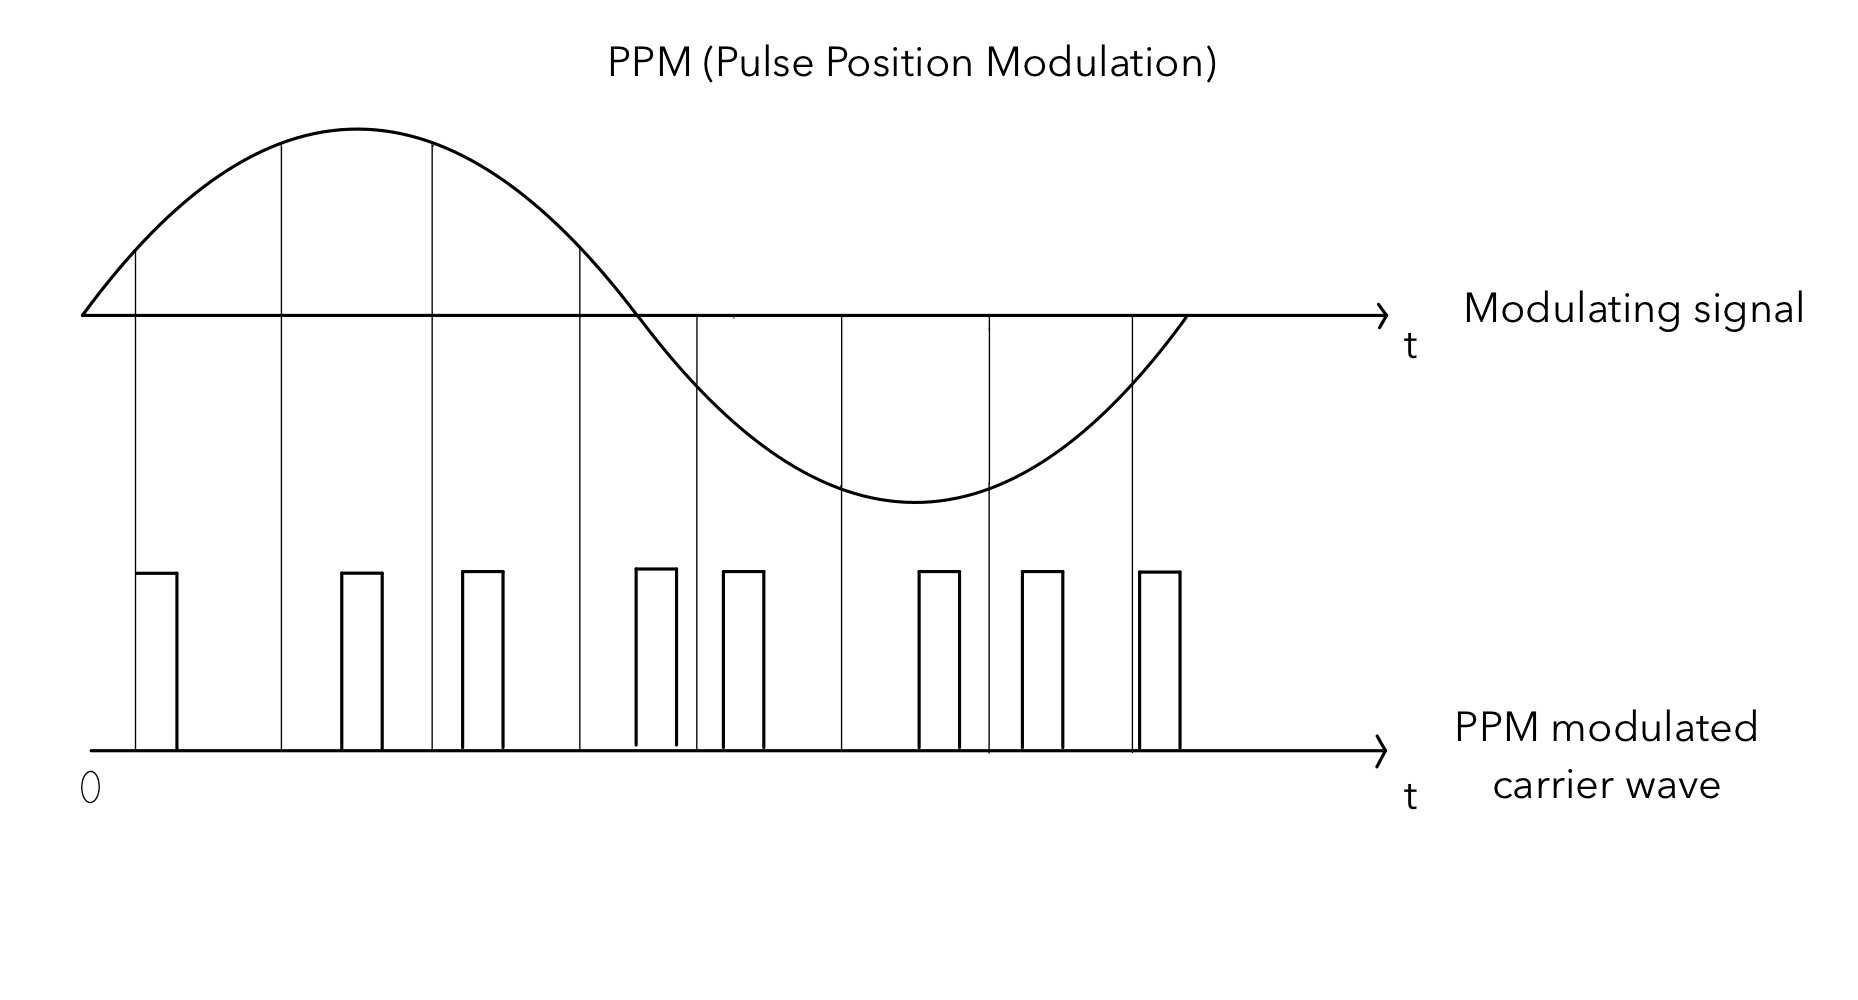
\includegraphics[width = 15cm]{Media/Document/ppm.png}
    \caption{Figure showing Pulse Position Modulation - amplitude and width of the carrier wave remains constant, with the position changing only}
    \label{ppm}
\end{figure}

\subsection{Data Transfer Protocol}

Just as protocols such as TCP/IP are required in Earth-based communications, data transfer protocols are required in space to specify how data should be transferred. These protocols must be suited for the unique challenges associated with deep space communications: regular communication outages, long distances resulting in large delays between sending and receiving signals, interference, etc. One such protocol is Delay/Disruption Tolerant Networking (DTN), developed and used by NASA. An advantage of DTN is that it allows for multiple hops between the sender and receiver, much like the Earth based internet \cite{dsnnasa}. One disadvantage of laser communications is that the beam is easily distorted in the atmosphere, for example by clouds. Other satellites could also serve as relays would mean that data can be gathered and held until atmospheric conditions improve, and then transmitted on to Earth. 

\section{The Near-Sun Environment}
\label{The Near-Sun Environment}

The Sun's core contains billions of nuclear fusion reactions that allows for the creation of hot plasma to be formed but this is not the only hazardous effect the Sun emits. The Sun is made up of multiple layers but the most important are the core, photosphere, chromosphere and the corona as depicted in \cref{TheSun}. The core contains Hydrogen and by nuclear fusion converts it into Helium. This creates a vast amount of energy that causes photons to form, leading to the visibility of the photosphere. This layer is visible to the naked eye and varies in temperature around 7,000 Kelvin causing its colour to shift. The chromosphere is split between its lower and upper region, both total to a thickness of around 2,000 km. Heated by the photosphere, it ranges in temperature between 4,300 - 10,200 Kelvin. These high temperatures cause gas to be ejected (solar flares). The last layer is the corona and its temperature ranges from 2 million - 5 million Kelvin, its still unknown what truly causes the corona to be so hot but the corona assists the plasma and highly charged particles of solar winds to be emitted into outer space and most importantly towards Earth \cite{TheSun}. \\

For decades scientists on Earth have witnessed and observed the effects the Sun has not only to the Earth itself, but to its spacecraft, most notably satellites. The high energy particles that are emitted from the Sun can damage materials on spacecraft and also penetrate through into the electronics causing a surge in power destroying microchips. Repeated exposure to these charged particles damage the chips, motherboards and most important solar panel equipment used to power these orbiting spacecrafts. Satellites are at higher risk to receive this exposure more than electronics based on the ground on Earth due to the lack of natural protection that Earth's environment offers against the hazards of the Sun. Other Earth based scenarios that are impacted by the Sun are the use of radio signals and navigation. Geomagnetic (solar) storms, charged particles emitted from the Sun's corona, disturb the Earth's magnetic field causing the ion sphere to deform. The radio signals that reflect off of this ion sphere are distorted, especially GPS signals. \\

The Sun's radiation encompasses the entire electromagnetic spectrum with a large proportion of UV, visible and infrared radiation. All of these types of radiation exist scattered throughout the Sun's environment, some travel with the solar wind and coronal mass ejections emitted from the Sun, but pose a significant risk to human life on Earth. However, spacecraft materials are not immediately affected by concentrated amounts of radiation. Research is still ongoing in this area of study, although so far indicates that exposure to radiation can cause mechanical and physical properties to change, particularly in non-metals. For metals such changes can be reversed by exposure to heat that causes their mechanical properties to return to normal \cite{DamageToMaterials}. \\

\begin{figure}[H]
\centering
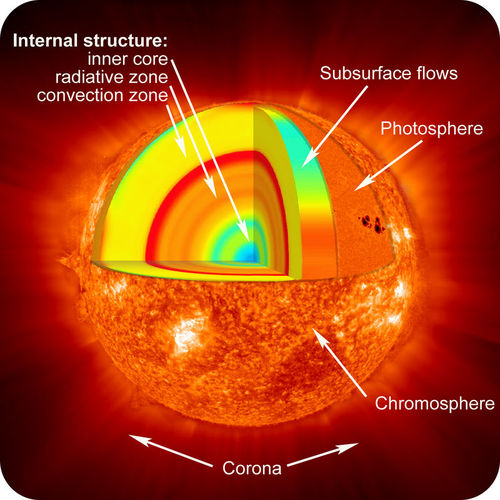
\includegraphics[scale=2.0]{Media/Document/201412291419879042243664_ce790b2e534a8859f7524dbfa6be7409-201412291419879560552576.jpg}
\caption{Figure depicting the layers of the Sun. Source \cite{TheSun}}
\label{TheSun}
\end{figure}

\section{Materials}
\label{Materials}

\begin{figure}[H]
\centering
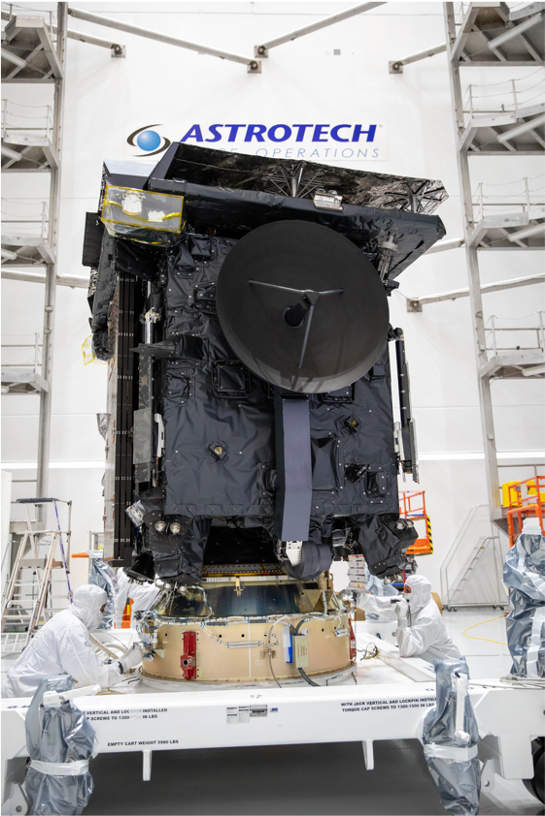
\includegraphics[scale=0.7]{Media/Document/Picture 1.png}
\caption{Image showing the heat shield on the Solar Orbiter spacecraft. Source \cite{SolarOrbiter}}
\label{SolarOrbiter}
\end{figure}

Materials for this mission must be heat resistant, radiation resistant and have low thermal conductivity, but must be able to function in space. The materials must have the ability to change with the temperature fluctuations, reform or hold their sizes and shapes, be able to withstand physical encounters with debris and have the durability, strength and a certain percentage of malleability to adapt to its surroundings without compromising structural integrity. The launching of such a spacecraft causes the materials to undergo shock via vibrations and the above criteria will allow the structure to hold as it escapes Earth's atmosphere. \\

As the spacecraft will be entering an orbit of less than 0.2AU of the Sun, it will need to resist many hazardous effects that the Sun outputs. The most significant effect is heat. When NASA (National Aeronautics and Space Administration) launched the Parker probe and ESA (European Space Agency) launched the Solar Orbiter probe, both were fitted with a heat shield not to repel heat, but to disperse it. The Parker probe had a thick foam core sandwiched between two carbon composites that was angled on one side of the probe that would always face the Sun so that the heat would travel along the heat shield and be expelled. For the solar orbiters heat shield shown in \cref{SolarOrbiter}, "The heat shield is built like a 10-foot-by-8-foot sandwich. The front layer — wafer-thin sheets of titanium foil — strongly reflects heat. A honeycomb-patterned aluminium base, covered in more foil insulation, forms the inner slice closest to the spacecraft and provides support" \cite{SolarOrbiter}. The front of the Solar Orbiter heat shield is covered by a layer of calcium phosphate that absorbs heat and forces it into channels that allows heat to escape through it, after which it gradual disperses by a titanium mirror, this allows the metal not to succumb to the full extent of the Suns heat to which prolongs its life and reduces changes in its mechanical properties. \\

The materials ideal for such a mission are one which have low thermal conductivity properties and high resistance to high temperatures, such properties are listed in \cite{CRC} to which titanium, steel and tungsten are shown to be ideal metals to be used alongside aluminium when used as an alloy. The use of non-metals such as Kevlar and carbon are also ideal due to their strength and heat resistance and most composite materials do not meet this mission's criteria as they will succumb to the heat or radiation found in the Sun environment outlined in \cref{The Near-Sun Environment}. The materials above undergo minimal effects from radiation but the electronics inside the spacecraft will be at risk of charged particles and interference from the radiation caused by the Sun's environment. Lead is ideal for resisting gamma radiation however not only is it heavy, it is soft and malleable and is able to deform under stress and can crack or break. Other materials that are suitable for resisting electromagnetic and other types of radiation are sheet metals formed from copper, brass and steel, though these materials have disadvantages in their weight, malleability and heat resistance \cite{CRC}. \\

\begin{figure}[H]
\centering
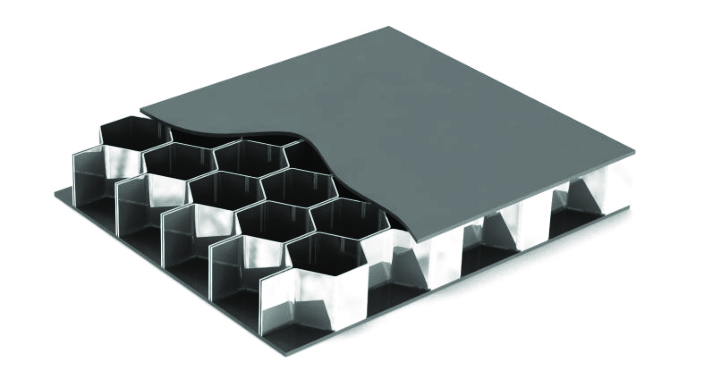
\includegraphics[scale=0.5]{Media/Document/Honeycomb-structure-Honeycomb-structures-are-highly-laborious-in-manufacturing-and.png}
\caption{Visual aid of the implementation of a honeycomb structure \cite{HoneycombPic}.}
\label{Honeycomb Image}
\end{figure}

\begin{figure}[H]
\centering
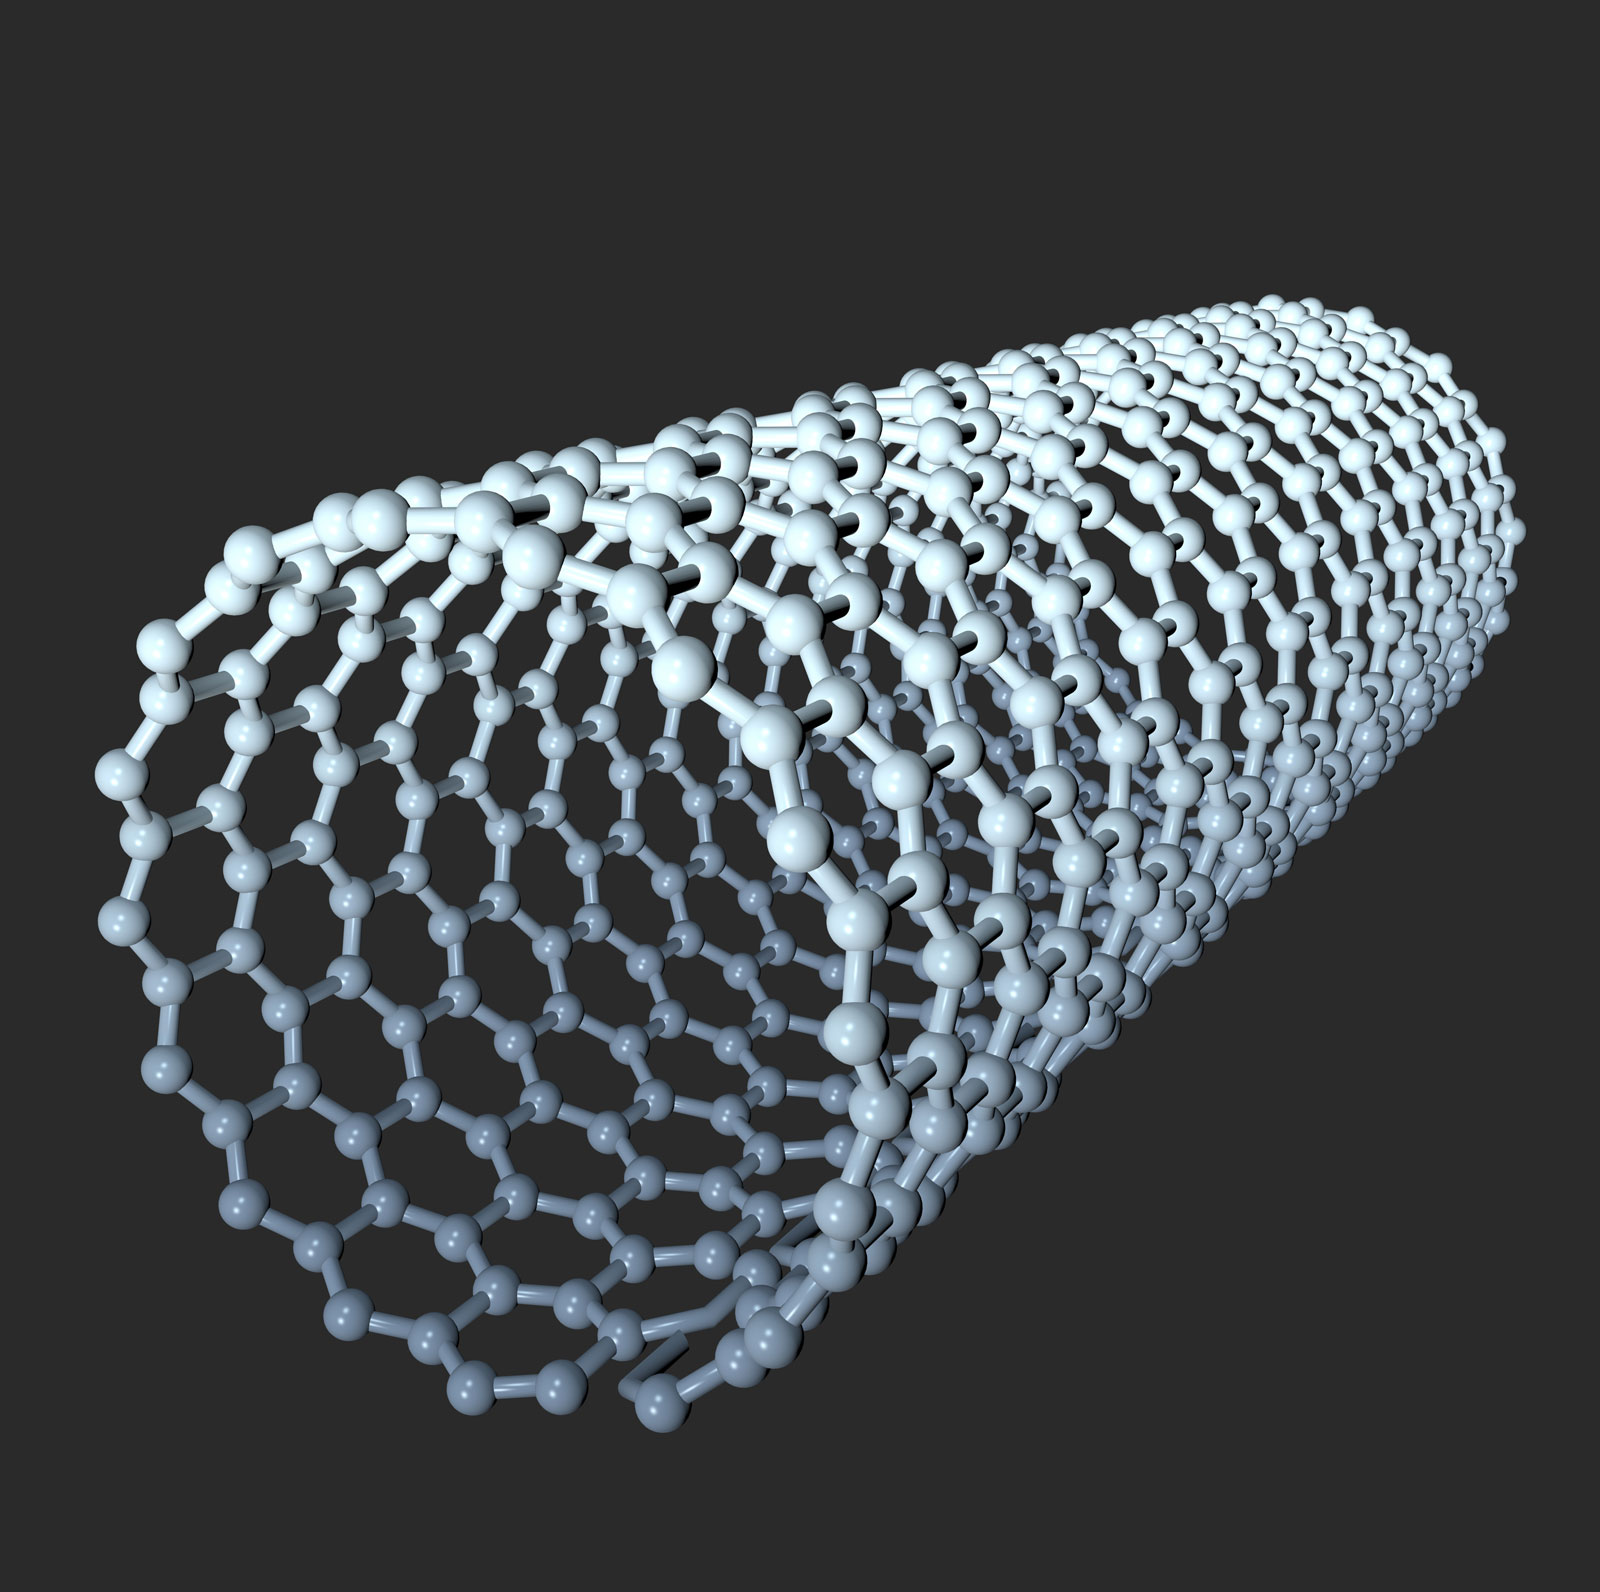
\includegraphics[scale=0.15]{Media/Document/Illustration-carbon-nanotube.jpg}
\caption{Illustration of a sheet of carbon nanotube \cite{CarbonNano}.}
\label{Carbon Nanotube image}
\end{figure}

The honeycomb structure used in the Solar Orbiter probe allows for an increase in strength while having low weight. The spacecraft total weight is an important factor when choosing materials as it affects the amount of fuel needed to leave Earth's atmosphere and how it orbits the Sun, the total weight is increased by the instruments and power supplies as well as all of the redundancy equipment on board so the structure and material choice is where the spacecraft has to save the most weight. Carbon nanotubes and honeycomb structures are two ideal countermeasures to an issue of weight, as both show an increase in high tensile strength, durability, lightweight properties and carbon nanotubes offer an increase in electrical and thermal resistance. \\

The use of a honeycomb structure is ideal when paired with other materials such as lead, steel, aluminium and iron, some of which are heavy materials that can replace the effect of strength and lower the weight \cite{Honey1}. Carbon nanotubes are beneficial as an improvement as multiple carbon nanotube sheets can be placed on the surface of a material and increase its thermal conductivity and tensile strength. A disadvantage though is that its expensive and time consuming to produce however this is a minimal effect when placed on a spacecraft that cannot be altered after it lifts off from Earth, though other materials and structures are available. \\

%--------------------------------------------------------------------------- 

%	CONCLUSION 

%--------------------------------------------------------------------------- 

\section{Conclusion} 

\label{Conclusion Section} 

This project has explored and discussed many aspects of a potential near sun exploration mission, including mission purpose, instrumentation, and communications. The proposed mission's purpose would be primarily to gather data on solar weather, such as CMEs (coronal mass ejections), solar maxima and minima, and the Sun's changing magnetic field. Whilst this investigation would be of great scientific value, particularly in the study of energetic solar particles, the mission could justify itself economically with the greater understanding of solar weather it could bring. Understanding what drives solar weather events might allow us to build models with predictive power, allowing us to mitigate the risk of damage to our Earth and space based equipment from power surges. In this way, answering questions about the dynamics of the near sun environment will simultaneously provide scientific and financial benefits. \\

Furthermore, understanding the Sun as a power source may provide insights into Earth based nuclear fusion technology. In order to collect this data the proposed probe would be equipped with a magnetometer (for measuring the magnetic fields around the Sun), a Faraday cup (for counting particles) a mass spectrometer (to identify isotopes) and a thermal gauge (to measure the temperature of the probe and its surroundings). The logistics of communication between the Earth and Sun has also been discussed - the possibility of using Deep Space Optical Communications as an alternative to traditional radio frequencies has been evaluated, and it was found that this could be a cost effective option but its efficacy will be dependent on mission specifics such as orbital eccentricity. Additionally, the technology is in the early stages of its development, so whether or not this could be used may depend on future test mission results.

\vspace{\baselineskip}

The spacecraft is advised to utilise a honeycomb structure as part of its heat shield to keep the overall mass down, while the use of aluminium, steel and titanium can offer protection against impacts and thermal damage. Steel and lead or copper may provide protection against the radiation that it will encounter. The spacecraft design would operate such that certain materials will reflect the heat and allow the interior of the spacecraft to remain cooler and as the interior must be protected from the radiation. Thermal resistant properties are not required for these materials. Nanotubes offer a lightweight, high strength and thermoresistant properties and can be used to line the external side of the main hull to offer an increase in heat resistant properties where needed. \\

This project was exclusively literature based as we can only base our research on data from previous missions. However, in the future, it would be useful to devise a simulation to test some simple features of the proposed probe in the near-Sun environment. For example, modelling the effect of extreme temperatures on the materials suggested for use, or simulating the regions in the probe's orbit where communications would or would not be possible. It was felt during this project that not enough specifics of the mission design were known to construct such a simulation, but with more time and information this would be an opportunity for further research. Due to the vast amount of relevant information to this project, further literature review would also be valuable.  

\vspace{\baselineskip}

Future research should investigate more specifically the logistics of the proposed mission. It should look at the orbit the solar probe should attain, as this affects the possibilities for communications and will determine what temperatures, and for how long, the probe would be exposed to. At this stage it was not known precisely to within what distance of the Sun the proposed probe would be able to travel safely. It should also provide a costing for the probe described in this report, by determining the approximate cost and mass of materials and instruments. It should also resolve some unanswered questions, such as whether optical communications would be a viable alternative to radio. This could be achieved with the help of simulations, and by comparing to the costs of previous similar missions such as the Solar Orbiter or the Parker Solar probe. Overall, this project has explored the topics it set out to and investigated the value of a very near-Sun mission and some of the ways in which this can be accomplished.

\newpage

%--------------------------------------------------------------------------- 

%	REFERENCES 

%--------------------------------------------------------------------------- 
\printbibliography
%--------------------------------------------------------------------------- 

%	APPENDIX 

%--------------------------------------------------------------------------- 

\newpage 

\section{Appendix} 
\label{Appendix Section} 

\subsection{Project Brief}
\label{project brief}

Background: \\

The Sun is an object of immense interest to astronomers and environmental scientists alike. As the central energy source powering our solar system, it is of critical importance to the lives of everything on Earth. Over the centuries it has been studied at length but there still remain considerable gaps in our understanding of the fundamental processes which take place within our nearest star. \\

Previous missions such as SOHO and Ulysses have provided the freedom to investigate the Sun and its environment away from the confines of Earth and its protective atmosphere and magnetosphere. The data from these spacecraft will soon be supplemented by Solar Orbiter which was launched earlier this year; a current M-Class mission candidate developed with ESA to investigate the Sun from as close as 0.28AU (62 solar radii). \\

However, even 0.28AU is a considerable distance from the Sun; this is not much nearer than the closest approach of Mercury. To fully understand the processes and dynamics of the Sun it will be necessary to one day approach even closer.  Only by experiencing in-situ the complex near-Sun environment can the mechanisms at work within the Sun begin to be unravelled
Aims and objectives: \\

The aim of this project is to investigate the scientific benefit of a very near-Sun mission and the technologies which are needed to enable this. In this context, “very near-Sun” refers to missions where the science phase should occur at anything from 0.2AU to 0AU. \\

You should consider: 
\begin{itemize}
    \item What data can be collected in the very near-Sun environment
    \item How this data shall be transmitted to and recived by Earth
    \item What instrumentation will be required on-board? Consider the technology readiness level.
    \item What will be the effects of a very near-Sun environment on a spacecraft and its instruments 
    \item How will the data collected be used? What are the technological/economic 
    \item The materials required to withstand the thermal and radiation environment, to protect both instrumentation and the spacecraft 
\end{itemize}

There is a wide variety of useful science that can be achieved at various distances from the Sun and a huge range of solutions to meet the resulting science requirements. You should not only consider  the scientific aims of the mission, but also the extremely challenging thermal and radiation environment that will place constraints on the mission. Discuss the innovative use of technologies and materials will be necessary to meet these demands. \\

Outputs expected:
\begin{itemize}
    \item Detailed analysis of the near-Sun environment (you may want to include a simulation) and the effects on spacecraft 
    \item A discussion of the data to be collected and the instrumentation required 
    \item Description of chosen data transmission technique and how it will be received by Earth 
    \item Reccomendations for protection against thermal, physical and radiation damage 
    \item Assessment of the technological and economic benefits of such a mission 
\end{itemize}

These outputs should be finalised in a technical report, additional models and simulations may also be submitted.  

\subsection{Project Outline}
\label{project outline}

Probes have been launched to study the Sun and near-sun environment since the 1950s, beginning with NASA's Pioneer probes \cite{pioneers}, and are still regularly launched today, most recently, the ESA solar orbiter. There are still many unanswered questions about our own sun - for example, why is the Sun's corona counter-intuitively hotter than its surface? What is the nature of the solar winds? Answering these questions and more will help us to further understand our own sun, and hence distant stars as well. Additionally, the sun is responsible for weather effects here on earth, such as satellite damage due to solar energetic particle events \cite{satellites}. Understanding these phenomena may allow us to mitigate their effects, with obvious economic benefits. 

\vspace{5mm}

Very close proximity to the sun is required to properly investigate the near sun environment. This introduces particular challenges to the mission - namely the heat generated near the sun. The sun's corona extends for 5 million miles, or approximately 12 solar radii from its core, and has temperatures in excess of 1 million Kelvin \cite{corona}. Probing near this region would require a spacecraft with extraordinarily heat resistant shielding. The effect of extreme temperatures on the spacecraft's instruments must also be taken in to account.

\vspace{5mm}

This project aims to investigate the theoretical feasibility of such a mission to between 0 and 0.2AU of the sun, and what benefits it could provide. It will investigate and discuss in detail what data the mission could aim to collect, and for what purposes, how this data will be communicated back to earth, and how the challenges associated with the inhospitable environment could be overcome. It will discuss both existing technology, and speculate on what innovation will be necessary to make such a mission possible. The aim is to produce: 

\begin{itemize}
    \item A background of previous missions in this area
    \item A discussion on the scientific and economic benefits of a very near sun mission
    \item An analysis of the near sun environment, and description of the shielding technology necessary to ensure the safety of the craft and its instruments
    \item A discussion, and analysis of the best way to transmit this data back to earth
\end{itemize}

Each team member will take responsibility for their own subtopic, which will be split into segments 1 and 2. This is to make sure than any segment 1 research by one team member that is a prerequisite for segment 2 research for another member is completed by a set date, allowing the second team member to continue working based off of the output from segment 1. The following Gantt chart details the schedule of work to be completed:

\subsection{Project Gantt Chart}
\label{Gantt Chart}

\begin{figure}[H]
\centering
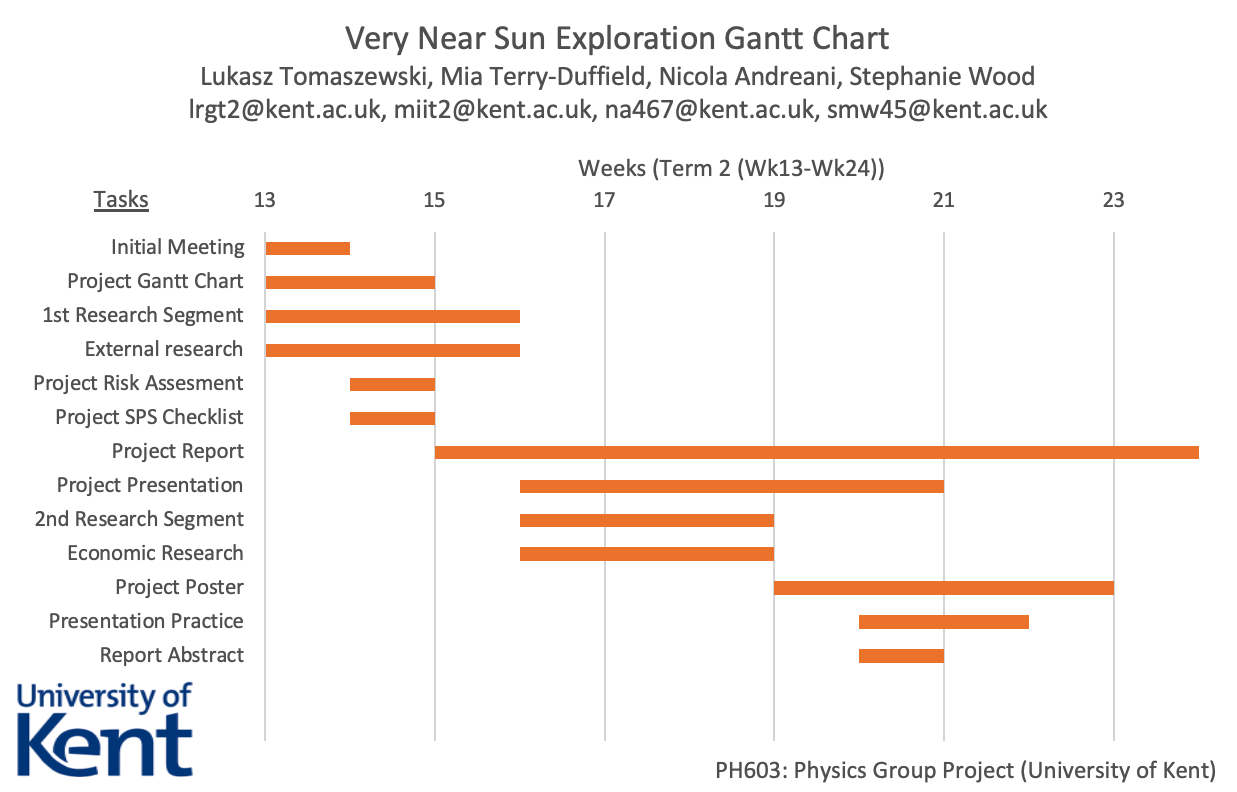
\includegraphics[width = 17cm]{Media/Document/gantt.png}
\caption{Gantt chart detailing project timeline}
\label{gantt}
\end{figure}

\subsection{Project Timeline}
\label{Project Timeline}

\textbf{\underline{Week 13:}} \\ [0.2cm]
Start research (all bullet points split between group members). Form Gannt chart. \\

\textbf{\underline{Week 14:}} \\ [0.2cm]
Confirm external research? Finalise Gantt chart and submit. Form report layout and structure. Discuss other factors to include beside research? (Mathematical proofing). Submit Gantt chart. Submit Risk assessment. Submit SPS checklist. \\

\textbf{\underline{Week 15:}} \\ [0.2cm]
Finalise research on first bullet point (submit for report analysis). Finalise report layout and structure.  Meeting aims to discuss progress and highlight problems. Confirm report structure and start drafting presentation. Economic research to be started. Submit Meeting minutes. \\

\textbf{\underline{Week 16:}} \\ [0.2cm]
Start research on second bullet point. First bullet point’s research including in report. Economic research to be started. Finalise presentation layout and structure. Form presentation based of current report structure. Read current report draft. Submit Meeting minutes. \\

\textbf{\underline{Week 17:}} \\ [0.2cm]
Finalise external research. Finish research on second bullet point. Analyse missing information. Read current report draft. Read current presentation draft. Economic research to be completed. V Mason’s opinions? Submit Meeting minutes.\\

\textbf{\underline{Week 18:}} \\ [0.2cm]
Read current report draft. Read current presentation draft. Assign presentation roles. Talk about group poster. Assist in report writing if needed (depending on in-house evaluation).
Submit Meeting minutes. \\

\textbf{\underline{Week 19:}} \\ [0.2cm]
Presentation to be near completion. Read current report draft. Read current presentation draft. Week 19 held as a buffer week to provide additional support time (if required.) Report discussion to be discussed (members have paragraph each or all members form the section as one?). Submit Meeting minutes. \\

\textbf{\underline{Week 20:}} \\ [0.2cm]
Presentation finalised and members allocated slides/ sections and or presentation to be corrected per analysis. Read current report draft. Start group poster. Finalise report abstract before submission. Submit Meeting minutes. \\

\textbf{\underline{Week 21:}} \\ [0.2cm]
Read current report draft. Report discussion either submitted to Mia or confirmed/ written in meeting? Report to be near completion. Group poster near completion. Practice presentation. Submit Report Abstract. \\

\textbf{\underline{Week 22:}} \\ [0.2cm]
Read current or final report draft. Finalise group poster before submission. Presentation Time. \\

\textbf{\underline{Week 23:}} \\ [0.2cm]
Read final report draft. Final confirmation. Submit Group Poster. \\


\textbf{\underline{Week 24:}} \\ [0.2cm]
Submit Final Project Report.

\subsection{Self-Appraisal}

%ii) a self-appraisal of your successes in terms of implementing your original plans and
%reaching your own planned milestones. This will address the functioning of the project team
%and will be a 1-2 page reflection on the way in which the team operated – it must be signed
%and dated by all team members. 

In our initial meeting, we set out our plan for the project and discussed which tasks would be required to compile a report on very near-Sun exploration. For this report to meet the project aims in the given outline, we would need to research several aspects of solar probe design, instruments and functions, the environment the probe would encounter and the desired outcome of such a mission. The research was divided between Nicky, Stephanie, Mia and Lukasz. The mission purpose and data collection sections were reviewed by Nicky, the history of solar probes and scientific instrumentation sections were managed by Stephanie, communications was handled by Mia, and the materials and very near-Sun environment research was assigned to Lukasz. Mia was responsible for organising and writing up each individual's research into the finalised report and compiling references in Latex based on URLs provided by other group members. Stephanie and Mia have copy edited the finalised report. The presentation for the project consisted of a PowerPoint slideshow, the slides for which were designed by Nicky and Lukasz, but all members of the group wrote up their own slides to ensure they were confident and knowledgeable subsequently talking in the presentation. We were also asked to design a poster summarising our research and findings on the very near-Sun probe. This was produced by Stephanie and vetted by Mia. \\

To summarise, the work was completed with the following distribution:

\begin{itemize}
    \item History of Solar Probes research - Stephanie Wood
    \item Instrumentation research - Stephanie Wood
    \item Poster - Stephanie Wood
    
    \item Mission Purpose research- Nicola Andreani
    \item Data Collection research - Nicola Andreani
    \item Presentation slide design - Nicola Andreani
    
    \item Presentation slide design - Lukasz Tomaszewski
    \item The Near-Sun Environment research - Lukasz Tomaszewski
    \item Materials research - Lukasz Tomaszewski
    \item Gantt Chart - Lukasz Tomaszewski
    
    \item Communications research - Mia Terry-Duffield
    \item Project Overview - Mia Terry-Duffield
    \item Final report write-up - Mia Terry-Duffield
    
\end{itemize}


\end{document} 